\documentclass[11pt]{article}
\usepackage[margin=1in]{geometry}
\usepackage{amsmath,amssymb,amsthm,mathtools}
\usepackage{booktabs,enumitem,graphicx,xcolor}
\usepackage{xurl}
\usepackage[section]{placeins}
\usepackage[colorlinks=true,linkcolor=blue!50!black,citecolor=green!35!black,urlcolor=blue!50!black]{hyperref}
\usepackage[nameinlink]{cleveref}
\newtheorem{theorem}{Theorem}\newtheorem{proposition}[theorem]{Proposition}\newtheorem{lemma}[theorem]{Lemma}\newtheorem{corollary}[theorem]{Corollary}
\theoremstyle{definition}\newtheorem{definition}[theorem]{Definition}\newtheorem{remark}[theorem]{Remark}\newtheorem{example}[theorem]{Example}
\newcommand{\R}{\mathbb R}\newcommand{\X}{\mathbb X}\newcommand{\C}{\mathcal C}
\newcommand{\lex}{\ge_{\mathrm{lex}}}
\setlength{\emergencystretch}{3em}
\title{A Tangent Structure for Injected Data:\\ Feasible Cones, Universality at Corners, Jets on the Tetrad Scheme,\\ and Decision Boundaries}
\author{Vinay K Awasthi\\ Johns Hopkins University\\ \texttt{vawasth1@jh.edu}}
\date{October 2026}
\begin{document}
\maketitle

\begin{abstract}
In the lab for latent actors \cite{Lab}, an adversary injects a share $\varepsilon\ge0$ of records from a law $Q$ into data from a truth
$P$. Every slope, stealth direction and obstruction in that paper is a statement about tangent vectors of the probability simplex. The lab
paper only named the tangent-category structure behind them. This companion builds it and checks every axiom on finite examples.
\begin{itemize}
\item \emph{The cone structure.} Take polyhedra and the lexicographic sets they generate, with affine maps; on simplices the affine maps
  are exactly the stochastic matrices. On this category the feasible-direction functor $T$ carries a projection, a zero, an addition, a
  vertical lift and a canonical flip satisfying every equational axiom of Cockett and Cruttwell \cite{CockettCruttwell2014}. Its additive
  bundles are commutative monoids, which have negatives only at relative-interior points. An injection direction $Q-P$ is exactly a
  tangent vector.
\item \emph{Universality fails exactly at the boundary.} The vertical lift is universal at a point if and only if the point lies in the
  relative interior. At a boundary point the fibre of $T(p)$ over the zero section contains $(x,u,0,-u)$ for every $u$ that enters the
  interior: a second-order direction may take back mass that the first-order direction has just placed. The fibre equals
  $C_x\times C_{x,u}$, where $C_{x,u}$ is the cone at ``$x$ moved infinitesimally along $u$''. Second-order functoriality also needs
  affinity: a polynomial self-map of $\Delta_3$ sends a point of $T^2\Delta_3$ outside it.
\item \emph{The lab's maps.} On the open simplex the usual tangent category applies. Theorem E's slopes are $T(F)(P,Q-P)$, and the
  stealth direction $\chi$ spans the vertical bundle of the marginal map. The decision pipeline is a morphism off the coincidence
  strata, where $|T\hat r|$ grows like $|v_2|^{-1}$. The value function is a morphism on each chamber; on a wall it fails to preserve
  addition by exactly the relevance functional $|\ell(\xi)|$.
\item \emph{Jets on the tetrad scheme.} With the Weil-algebra tangent structure the vertical lift is universal everywhere, even at
  singular points. What fails instead is completing a pair in $T_2V$ to a point of $T^2V$. The obstruction is the class
  $[H(u,v)]\in\operatorname{coker}J$. It vanishes off the two-coincidence stratum, and on it it has norm $|q(u,v)|/\sqrt2$ for an
  explicit quadric $q$. Its diagonal is twice the André--Quillen obstruction of the lab's Theorem G(4), so that obstruction is now a
  statement about $T^2$.
\item \emph{Using it on decision boundaries.} A smooth map of simplices is a second-order morphism at a corner iff each vanishing
  output cell has a Hessian that is bilinearly non-negative on a cone of null directions (\cref{thm:nonaffine}). Bayesian conditioning,
  stochastic matrices and products qualify. The lab's post-probe decision boundary is curved both ways. So two data sets that each lead
  to the same act can, pooled, lead to the other. This is impossible for affine decisions, and curvature forces it
  (\cref{prop:pool}). The 2-jet of the decision gives second-order attack budgets that can reverse the first-order verdict.
\item \emph{Layers.} At corners we keep layered maps with restriction criteria: strata, resolutions and multi-maps. Each open face is a
  tangent category, and the corner's universality failure is exactly a change of layer (\cref{thm:layers}). Blowing up resolves the
  coincidence and the merge. The explanation multi-map has corners where its domain ends and branches that die at positivity walls.
\item \emph{Restriction, sheets and global pooling.} The partial maps form a restriction category with joins, and $T$ is a restriction
  functor (axioms checked on $600$ laws). The tangent structure on a hiding sheet is the sheet's tangent cone, and it certifies worst-case
  decisions. Along any chord, pooling is decided exactly by two polynomials of degree at most six. Globally, pooling fails by leaving the
  domain, because the pooled covariances take the liar's sign class, and the flips that occur sit next to these holes.
\end{itemize}
The construction gives a dichotomy. Positivity breaks universality of the lift, and the algebra breaks completion to second order. This
parallels the lab's finding that real descent fails only through positivity. Fourteen checks (TG1--TG13 and TG6b) verify everything
exactly or to rounding, seven more (TD1--TD7) the decision-boundary results, eight (LY1--LY8) the layers, and eleven (RC, SH, GP) the restriction structure,
the sheets and global pooling.
\end{abstract}

\tableofcontents

\section{Introduction}\label{sec:intro}
The lab paper \cite{Lab} works on the simplex $\Delta=\Delta_n$ of laws on $n$ cells. An adversary who injects whole records moves the
observed law to $P_\varepsilon=(1-\varepsilon)P+\varepsilon Q$. Three of its results are first- and second-order statements.
\begin{itemize}
\item \emph{Theorem E(2), slopes.} $\frac{d}{d\varepsilon}F(P_\varepsilon)|_0=\sum_xQ(x)\,\mathrm{IF}(x)$.
\item \emph{Theorem F, the hidden channel.} The injections invisible to every pair table are $P+s\chi$ on a segment.
\item \emph{Theorem G(4), obstruction.} At $m=4$ variables a first-order tetrad-stealthy direction extends to second order iff an
  André--Quillen class vanishes.
\end{itemize}
The lab paper stated these as a correspondence with tangent categories \cite{CockettCruttwell2014}; this paper turns the correspondence
into a construction. The reviewer's challenge was to build the tangent structure rather than name it. We take ``build'' in the strict
sense: we give the objects, the functor and the five natural transformations, and check every axiom, the universality of the vertical
lift included, on $\Delta_3$, $\Delta_4$ and a non-simplex polytope. The universality check is a finite pullback computation.

Three structures appear, and they fail in complementary ways.
\begin{center}\small
\begin{tabular}{p{0.33\textwidth}p{0.12\textwidth}p{0.2\textwidth}p{0.2\textwidth}}\toprule
& equational axioms & vertical lift universal & $T^2\to T_2$ onto\\\midrule
cone structure on polyhedra (\cref{thm:cone}) & yes & only at relative-interior points & yes\\
open simplex, smooth maps (\cref{sec:interior}) & yes & yes & yes\\
Weil structure on the tetrad scheme (\cref{thm:scheme}) & yes & yes, also at singular points & not on the two-coincidence stratum\\\bottomrule
\end{tabular}
\end{center}
The lab's semialgebraic model, the tetrad scheme cut by positivity, has both failures. The first is a positivity phenomenon at
corners; the second is an algebraic phenomenon at singular points.

\section{Tangent structures and Weil algebras}\label{sec:defs}
\begin{definition}[Rosický \cite{Rosicky1984}; Cockett and Cruttwell \cite{CockettCruttwell2014}]\label{def:tangent}
A \emph{tangent structure} on a category $\X$ consists of an endofunctor $T$ and natural transformations
$p:T\Rightarrow1$, $0:1\Rightarrow T$, $+:T_2\Rightarrow T$, $\ell:T\Rightarrow T^2$ and $c:T^2\Rightarrow T^2$. Here $T_nM$ is the
pullback of $n$ copies of $p_M$; these pullbacks must exist and be preserved by every $T^m$. The axioms are:
\begin{enumerate}[label=(T\arabic*)]
\item $(p,+,0)$ makes each $p_M$ a commutative monoid in $\X/M$, the \emph{additive bundle};
\item $(\ell,0)$ is a morphism of additive bundles $(p,+,0)\to(Tp,T{+},T0)$;
\item $(c,1)$ is a morphism of additive bundles $(Tp,T{+},T0)\to(p_T,{+}_T,0_T)$;
\item $c\circ c=1$ and $c\circ\ell=\ell$;
\item $\ell_T\circ\ell=T(\ell)\circ\ell$, \ $c_T\circ T(c)\circ c_T=T(c)\circ c_T\circ T(c)$, and $c_T\circ T(c)\circ\ell_T=T(\ell)\circ c$;
\item \emph{universality of the vertical lift}: with $\nu=T(+)\circ\langle\ell\pi_1,0_T\pi_2\rangle:T_2M\to T^2M$, the square
\[
\begin{array}{ccc}
T_2M&\xrightarrow{\ \nu\ }&T^2M\\
{\scriptstyle p\pi_1}\downarrow&&\downarrow{\scriptstyle T(p)}\\
M&\xrightarrow{\ 0\ }&TM
\end{array}
\]
is a pullback, preserved by every $T^m$.
\end{enumerate}
\end{definition}

Leung \cite{Leung2017} showed that a tangent structure is an action of the Weil algebras
$W_k=\R[e_1,\dots,e_k]/(e_1^2,\dots,e_k^2)$ and their tensor products. This gives a uniform coordinate system that we use throughout; Garner \cite{Garner2018} shows every tangent category embeds in one of this Weil-algebra kind. A point
of $T^kM$ over $x$ is an element
\[
X=\sum_{S\subseteq\{1,\dots,k\}}c_S\,e^S,\qquad c_\varnothing=x,
\]
where $e_1$ is the innermost $T$ and $e_k$ the outermost. For example, $x+a\,e_1+b\,e_2+d\,e_1e_2\in T^2M$ is the tangent vector $(b,d)$ at
the point $(x,a)$ of $TM$. Every structure map is a substitution of generators:
\begin{center}\small
\begin{tabular}{lll}\toprule
map & on $T^kM$ & substitution\\\midrule
$T^ap\,T^b$ & $T^kM\to T^{k-1}M$ & $e_{b+1}\mapsto0$\\
$T^a0\,T^b$ & $T^kM\to T^{k+1}M$ & insert a new generator at position $b+1$\\
$T^a\ell\,T^b$ & $T^kM\to T^{k+1}M$ & $e_{b+1}\mapsto e_{b+1}e_{b+2}$, outer generators shifted up\\
$T^ac\,T^b$ & $T^kM\to T^kM$ & $e_{b+1}\leftrightarrow e_{b+2}$\\
$T^a({+})T^b$ & $T^a(T_2)T^bM\to T^kM$ & the two summand generators $\mapsto$ one generator (their product dies)\\\bottomrule
\end{tabular}
\end{center}
In these coordinates
\[
\ell(x,v)=(x,0,0,v),\qquad c(x,a,b,d)=(x,b,a,d),\qquad \nu(x,a,d)=(x,d,0,a)\quad\text{(order $1,e_1,e_2,e_1e_2$)}.
\]
The equational axioms (T4)--(T5) and the additivity parts of (T2)--(T3) are identities between substitutions. Check TG3 verifies all
eleven on random coefficient arrays. What remains for any given category is that the maps \emph{land in the right sets} (for
the cone structure), and the universality (T6). For a smooth $f$, $T^k(f)$ is $f$ evaluated on $W_k$-valued arguments. This is forward
differentiation with hyper-dual numbers; check TG1 confirms it against finite differences, and the symmetry of the $e_1e_2$ coefficient
(Schwarz) is naturality of $c$.

\section{The cone structure on polyhedra}\label{sec:cone}
\subsection{Lexicographic sets}
For $z\in X\subseteq\R^N$, the \emph{feasible directions} are
\[
D_X(z)=\{u:\ z+tu\in X\text{ for all }t\in[0,t_0]\text{, some }t_0>0\},
\]
and $TX=\{(z,u):z\in X,\ u\in D_X(z)\}$ \cite[Chapter 6]{RockafellarWets1998}. For an affine map $f$ with linear part $L$, $Tf(z,u)=(f(z),Lu)$. For the simplex,
$D_\Delta(x)=C_x=\{u:\sum u=0,\ u_y\ge0\text{ where }x_y=0\}$. For $x=P$ this is exactly the set of injection directions:
$C_P=\operatorname{cone}\{Q-P:Q\in\Delta\}$.

Write $(t_1,\dots,t_L)\lex0$ when the first non-zero entry is positive, or there is none. A \emph{lexicographic set} is a subset of some
$\R^N$ cut out by finitely many affine equations and finitely many conditions $(f_1(z),\dots,f_L(z))\lex0$ with affine $f_i$. Polyhedra are
the case $L=1$. Let $\C$ be the category of lexicographic sets and affine maps between them, an affine map $\R^N\to\R^{N'}$ sending $X$
into $X'$.

\begin{lemma}[interleaving]\label{lem:interleave}
Let $X=\{z:(f_1(z),\dots,f_L(z))\lex0\}$ with $f_i$ affine with linear parts $F_i$. Then
\[
TX=\bigl\{(z,u):\ (f_1(z),\dots,f_L(z))\lex0\ \text{and}\ (f_1(z),F_1u,f_2(z),F_2u,\dots,f_L(z),F_Lu)\lex0\bigr\}.
\]
Hence $T$ maps $\C$ to $\C$. Its fibres $D_X(z)$ are convex cones, and $T$ preserves finite products and fibre products over affine maps.
\end{lemma}

\begin{proof}
Let $z\in X$ and let $j$ be the first index with $f_j(z)\ne0$ (so $f_j(z)>0$), or $j=L+1$. For small $t>0$ the tuple at $z+tu$ is
$(tF_1u,\dots,tF_{j-1}u,\ f_j(z)+tF_ju,\dots)$. Its entry $j$ stays positive, so it is $\lex0$ iff $(F_1u,\dots,F_{j-1}u)\lex0$.
This is exactly the interleaved condition, because the $f_i(z)$ with $i<j$ vanish and $f_j(z)>0$ decides. A lexicographic cone is
closed under sums and positive multiples, so the fibres are convex cones. For products and fibre products, take the smaller of the two
thresholds $t_0$; an affine equation $g(z)=h(z')$ holds along $(z,z')+t(u,u')$ iff it holds at $t=0$ and $Lg\,u=Lh\,u'$. The set fibre
products are the categorical ones in $\C$, because a map into them is a pair of affine maps.
\end{proof}

Iterating the lemma on the half-line $H=\R_{\ge0}$ gives one condition for each subset $U$ of the generators.

\begin{lemma}[the lexicographic lemma]\label{lem:lex}
A point $\sum_Sc_Se^S$ lies in $T^kH$ iff, for every $U\subseteq\{1,\dots,k\}$, the coefficients $(c_S)_{S\subseteq U}$ are
$\lex0$ when the monomials are listed in decreasing size. The size order takes $e_1\ll e_2\ll\cdots\ll e_k\ll1$: $e^S$ precedes $e^{S'}$
iff the smallest generator of $S\,\triangle\,S'$ lies in $S'$. For $k=2$ and $U=\{1,2\}$ the order is $(1,e_2,e_1,e_1e_2)$, so the conditions
are
\[
c_\varnothing\ge0,\quad(c_\varnothing,c_1)\lex0,\quad(c_\varnothing,c_2)\lex0,\quad(c_\varnothing,c_2,c_1,c_{12})\lex0 .
\]
$T^k\Delta$ is the set of $W_k$-points satisfying the equations ($\sum_yc_\varnothing(y)=1$ and $\sum_yc_S(y)=0$ for $S\ne\varnothing$)
and these conditions for every cell $y$. The same holds for any polyhedron, row by row.
\end{lemma}

\begin{proof}
Induction on $k$ with \cref{lem:interleave}. Apply $T$ with the new generator $e_k$. Each existing condition for $U$ is kept (the base
point) and acquires a companion for $U\cup\{k\}$, in which each $c_S$ is followed immediately by $c_{S\cup\{k\}}$. This interleaving is
the size order, because $e^S\gg e^{S\cup\{k\}}\gg e^{S'}$ whenever $e^S\gg e^{S'}$ in the order for $U$. The simplex is the preimage of
$H^n$ under an affine embedding, and $T$ commutes with affine preimages and intersections. Check TG2 verifies the lemma against the
definition, computed exactly with nested rational parameters, on all $3^{2^k}$ points of $\{-1,0,1\}^{2^k}$ for $k=1,2,3$. The
lemma's sets have $5$, $38$ and $2696$ members.
\end{proof}

\subsection{The theorem}
\begin{theorem}[the cone structure]\label{thm:cone}
On $\C$, the feasible-direction functor $T$ with
\begin{gather*}
p(z,u)=z,\qquad 0(z)=(z,0),\qquad (z,u)+(z,v)=(z,u+v),\\
\ell(z,u)=(z,0,0,u),\qquad c(z,a,b,d)=(z,b,a,d)
\end{gather*}
has the following properties.
\begin{enumerate}
\item[(1)] $T$ is an endofunctor, the $T_n$ exist and are preserved by every $T^m$, and all five maps are well defined and natural.
\item[(2)] Each $p_X$ is an additive bundle in commutative monoids. The fibre $C_x$ of a polyhedron is a group iff $x$ lies in the
  relative interior; otherwise there is $u\in C_x$ with $-u\notin C_x$.
\item[(3)] (T2)--(T5) hold.
\item[(4)] Let $X$ be a polyhedron. The vertical lift is universal at $x$, meaning the fibre of $T(p)$ over $0(x)$ equals $\nu(T_2X)_x$,
  iff $x\in\operatorname{relint}X$. In general that fibre is
\begin{gather*}
\{(x,u,0,w):\ u\in C_x,\ w\in C_{x,u}\},\\
C_{x,u}=\{w:\ \textstyle\sum w=0,\ g_rw\ge0\text{ for every active row $r$ with }g_ru=0\},
\end{gather*}
  and $C_{x,u}\supsetneq C_x$ whenever $g_ru>0$ for some active row $r$, that is, whenever $u$ moves off an active facet. So (T6) holds
  at relative-interior points and fails at every boundary point; it holds globally only on affine subspaces.
\end{enumerate}
\end{theorem}

\begin{proof}
(1) Functoriality is the chain rule for affine maps. The pullbacks exist and are preserved by \cref{lem:interleave}. The map $\ell$
lands in $T^2X$: $(x,0)\in TX$, and $(x,0)+s(0,u)=(x,su)\in TX$ since $C_x$ is a cone. The map $c$ lands in $T^2X$ because, by
\cref{lem:interleave} applied twice, $T^2X$ is cut out row by row by
\[
f\lex0,\quad(f_i,F_ia)_i\lex0,\quad(f_i,F_ib)_i\lex0,\quad(f_i,F_ib,F_ia,F_id)_i\lex0 .
\]
The first three are symmetric in $a,b$. For the last, let $j$ be the first index with $f_j\ne0$ and $i_0<j$ the first index with
$(F_ia,F_ib)\ne(0,0)$. The second and third conditions make the first non-zero of $F_{i_0}a$ and $F_{i_0}b$ positive, so the last
condition holds in either order. If there is no such $i_0$, the tuple reduces to $(F_1d,\dots,F_{j-1}d,f_j,\dots)$ in either order.
The other maps are restrictions of linear maps, so naturality for affine morphisms is immediate. Addition lands in $TX$ because fibres
are convex cones.

(2) For a polyhedron, $C_x$ is the polyhedral cone of the active rows. It is a linear subspace iff no active inequality is strict for
some direction, which means $x$ is relatively interior.

(3) These are substitution identities (\cref{sec:defs}) together with (1).

(4) For a row $g\cdot z\ge h$, the conditions on $(x,u,0,w)$ are $gx-h\ge0$, $(gx-h,gu)\lex0$ and $(gx-h,0,gu,gw)\lex0$. For an
active row with $gu=0$ this forces $gw\ge0$; with $gu>0$ it allows any $w$. This is the displayed fibre, and $\nu$ hits exactly
$C_x\times C_x$. If $x$ is relatively interior every active row is an implicit equation, $gu=0$ always, and the two agree. Otherwise
pick an active row and $u\in C_x$ with $gu>0$. Then $w=-u$ lies in $C_{x,u}$ but not in $C_x$, and the family $x+tu+st(-u)=x+t(1-s)u$
stays in $X$ for $0\le s<1$. The set fibre is the categorical pullback in $\C$, because the one-point set is an object and its maps
to $X$ are the points of $X$. So the square is not a pullback.
\end{proof}

\begin{remark}[what the failure says]
At a boundary point the vertical directions over $u$ are not those of the base. They are those of the face that $x$ enters when moved
infinitesimally along $u$. In injection terms, once a first-order injection has put mass on an empty cell, a second-order correction
may remove it again. The universal object is the bundle of cones $C_{x,u}$, not $T_2X=TX\times_XTX$. The addition needs $T_2X$, so the
cone structure cannot have both. Check TG6 confirms (4) by exact enumeration on $\Delta_3$ and $\Delta_4$ at every face type, and TG6b on
the cube cut by $x_1+x_2+x_3\le2$, where the fibre has $405$, $225$, $125$ and $104$ grid points against $324$, $144$, $64$ and $49$ at a
facet, an edge, a vertex and a cut vertex, with $729=729$ at the interior.
\end{remark}

\begin{proposition}[morphisms]\label{prop:morph}
\begin{enumerate}
\item[(1)] The affine maps $\Delta_n\to\Delta_m$ are exactly the stochastic matrices, the morphisms of $\mathrm{FinStoch}$
  \cite{Fritz2020}. They preserve every $T^k\Delta$, as does the product of laws $(x,y)\mapsto x\otimes y$ (checked, TG5).
\item[(2)] Smooth maps of simplices need not be morphisms at second order. The map $f(q)=(1-(q_1-q_2)^2,\ (q_1-q_2)^2,\ 0)$ sends
  $T\Delta_3$ into $T\Delta_3$, but at the vertex $x=(1,0,0)$ it sends
  $X=x+(-1,0,1)e_1+(-1,1,0)e_2\in T^2\Delta_3$ to a point whose cell-$1$ coefficients are $(0,0,0,-2)$, which is not $\lex0$.
\end{enumerate}
\end{proposition}

\begin{proof}
(1) An affine map of simplices sends vertices to laws, so its matrix is stochastic. A non-negative combination of $\lex0$ sequences is
$\lex0$, and this holds for every $U$. (2) The cell-$1$ coordinate is $(q_1-q_2)^2$. On $X$ the difference $q_1-q_2$ has coefficients
$(0,-1,1,0)$, so its square has $e_1e_2$ coefficient $2(-1)(1)=-2$ and nothing before it. The first-order part vanishes because
$f$ is critical at $x$, and $X$ itself satisfies \cref{lem:lex} (cells $1,2$: $(0,1,0,0)$ and $(0,0,1,0)$ in the order
$(1,e_2,e_1,e_1e_2)$).
\end{proof}

So at corners the honest morphisms are the Markov kernels, and the cone structure is a tangent structure on $\mathrm{FinStoch}$ in every
respect except (T6). This is where the lab's Markov-category reading \cite[Section ``Markov categories'']{Lab} and its tangent reading meet.

\section{The open simplex: the lab's maps are morphisms}\label{sec:interior}
On open subsets of affine spaces with smooth maps the tangent structure is the classical one, with $TU=U\times V$. It satisfies (T1)--(T6)
because it is a full subcategory of smooth manifolds \cite{CockettCruttwell2014}. The content lies in which of the lab's maps are
morphisms, and where. Write $\chi=\chi_{ABC}$ for the Walsh character and $K$ for the map to the three pair tables.

\begin{proposition}[the lab in the interior category]\label{prop:interior}
Let $m=3$, $P$ in the open simplex.
\begin{enumerate}
\item[(1)] \emph{Theorem E(2) is $T$.} For smooth $F$, $T(F)(P,Q-P)=\sum_xQ(x)\mathrm{IF}(x)$, with $\mathrm{IF}(x)=T(F)(P,\delta_x-P)$.
\item[(2)] \emph{Stealth is vertical.} The vertical bundle $\ker T(K)$ at $P$ is the line spanned by $\chi$. At the ends $s_\pm$ of
  the stealth range, $P+s_\pm\chi$ is a boundary point. There the cone structure gives the inward ray, and $T$ of the fibre is the same
  ray, so $T$ preserves the fibre pullback even at its ends.
\item[(3)] \emph{The pipeline is a morphism off the strata.} $\hat r=m_T/v_T$ with $v_T=\pm\sqrt{M_{01}M_{02}M_{12}}$ is smooth on
  $\{M_{01}M_{02}M_{12}>0\}$, and so is $P\mapsto U_a(\hat r(P))$. On approach to a coincidence $v_i\to0$, $\|T\hat r\|$ grows like
  $|v_i|^{-1}$.
\item[(4)] \emph{Walls.} The value $V=\max_aU_a$ of finitely many affine utilities is a morphism on each open chamber. At a point of the
  wall between $a$ and $b$ its directional derivative $DV(P;\xi)=\max(\ell_a\xi,\ell_b\xi)$ is positively homogeneous but not additive:
\[
DV(P;\xi)+DV(P;-\xi)-DV(P;0)=|\ell(\xi)|,\qquad \ell=\ell_a-\ell_b .
\]
  So the defect of the natural transformation $+$ is the relevance functional of the lab's Theorem L(4), and it vanishes iff $\xi$ is
  parallel to the wall.
\end{enumerate}
\end{proposition}

\begin{proof}
(1) $T(F)(P,\cdot)$ is linear, and $Q-P=\sum_xQ(x)(\delta_x-P)$. (2) $K$ is linear, and its kernel on zero-sum directions is one-dimensional,
spanned by $\chi$ (Theorem F(1) of \cite{Lab}). At $s_+$ some cell with $\chi<0$ is empty, so only $-\chi$ is feasible; at $s_-$
only $+\chi$. (3) Quotients and square roots are smooth where defined. With $M_{ij}=v_iv_j$, $\partial\hat r$ contains
$m_T\,\partial(v_T^{-1})$, and $v_T^{-1}$ has a simple pole along $v_i=0$. (4) This is Danskin's theorem \cite{Danskin1967} for a
maximum of two affine functions that are equal at $P$: $\max(\alpha,\beta)+\max(-\alpha,-\beta)=|\alpha-\beta|$.
\end{proof}

On the lab's worked example, $\hat r=-0.408$ and $T\hat r(P,\chi)=1/v_T=-157.50$, exactly Theorem F(2)'s rate. The $e_1e_2$ coefficient of
$T^2\hat r(P,\chi,\chi,0)$ is $0$: along the hidden channel $\hat r$ is affine. The wall between the two acts lies at $s=0.001$ on the pair
line, and $\ell(\chi)=-1$ there, so the additivity defect along $\chi$ is $1$ (checks TG8--TG10; \cref{fig:jets}(a)).

\section{Second order: the tetrad scheme}\label{sec:scheme}
For $m=4$ the lab's model lies in the scheme $V=\{T_1=T_2=0\}$ of the tetrads $T_1=M_{01}M_{23}-M_{02}M_{13}$ and
$T_2=M_{01}M_{23}-M_{03}M_{12}$, inside the affine hyperplane $\sum P=1$ of $\R^{16}$. Weil functors give it a tangent structure: $T^kV$
is the set of $W_k$-points of $V$ \cite{Weil1953,KolarMichorSlovak1993,Leung2017}. Equivalently, the opposite of commutative algebras
carries the tangent structure $TA=\operatorname{Sym}_A\Omega_A$ \cite{CockettCruttwell2014}. Concretely, for $J$ the Jacobian and $H$ the
full second derivative of $(T_1,T_2)$ at $P$,
\[
(P,a,b,d)\in T^2V\iff Ja=0,\ Jb=0,\ Jd+H(a,b)=0 ,
\]
because $T(P+ae_1+be_2+de_1e_2)=T(P)+Ja\,e_1+Jb\,e_2+(Jd+H(a,b))\,e_1e_2$ in $W_2$.

\begin{theorem}[jets on the tetrad scheme]\label{thm:scheme}
\begin{enumerate}
\item[(1)] \emph{Universality holds everywhere.} The fibre of $T(p)$ over $0(P)$ is $\{(P,u,0,w):Ju=Jw=0\}=\nu(T_2V)$ at every point,
  singular or not.
\item[(2)] \emph{Completion is obstructed.} The map $(p_T,Tp):T^2V\to T_2V$, $(P,a,b,d)\mapsto(a,b)$, has image
  $\{(a,b):[H(a,b)]=0\text{ in }\operatorname{coker}J\}$. At the lab's generic and one-coincidence truths $J$ has rank $2$ and the map
  is onto. On the two-coincidence stratum ($v_2=v_3=0$) $J$ has rank $1$, its cokernel is spanned by $T_1-T_2$, and
\begin{gather*}
\bigl\|[H(a,b)]\bigr\|=\tfrac1{\sqrt2}\,|q(a,b)|,\\
q(a,b)=dM_{03}(a)\,dM_{12}(b)+dM_{03}(b)\,dM_{12}(a)-dM_{02}(a)\,dM_{13}(b)-dM_{02}(b)\,dM_{13}(a).
\end{gather*}
  The image is the polarised quadric $\{q=0\}$.
\item[(3)] \emph{2-jets and Theorem G(4).} The 2-jets are the points $P+A\varepsilon+B\varepsilon^2$ of $V$ over $\R[\varepsilon]/(\varepsilon^3)$. They
  correspond, through $\varepsilon\mapsto e_1+e_2$, to the $c$-fixed points $(P,A,A,2B)$ of $T^2V$. So $A$ extends to a bent injection iff
  $[H(A,A)]=0$. This class is twice the obstruction $\mathrm{ob}(A)=[\tfrac12H(A,A)]$ of the lab's Theorem G(4). A direction with
  $\mathrm{ob}(A)\ne0$ is the velocity of no $C^2$ curve in $V$.
\end{enumerate}
\end{theorem}

\begin{proof}
(1) Put $b=0$ in the display: $H(u,0)=0$, so the conditions are $Ju=0$ and $Jw=0$. (2) Given $Ja=Jb=0$, a completing $d$ exists iff
$H(a,b)\in\operatorname{im}J$. On the two-coincidence stratum both rows of $J$ equal $M_{01}\,dM_{23}$, as in the proof of the lab's Theorem
G(3). So the unit cokernel vector is $(1,-1)/\sqrt2$, and the class is $(H_1-H_2)(a,b)/\sqrt2$. Since $T_1-T_2=M_{03}M_{12}-M_{02}M_{13}$
and the four covariances vanish there, its second derivative is the polarisation $q$. (3) The map $\R[\varepsilon]/(\varepsilon^3)\to W_2$,
$\varepsilon\mapsto e_1+e_2$, is an algebra map, because $(e_1+e_2)^2=2e_1e_2$ and $(e_1+e_2)^3=0$. It sends $P+A\varepsilon+B\varepsilon^2$ to
$P+A(e_1+e_2)+2Be_1e_2$. In characteristic zero, the points with $a=b$ are exactly its image. A $C^2$ curve in $V$ with velocity $A$ gives a
2-jet.
\end{proof}

Check TG11 finds a fibre of dimension $2\dim\ker J$ at all three truths: $26=2\cdot13$, $26$ and $28=2\cdot14$. Check TG12 finds every
random pair completable at the first two truths, and the class equal to $|q|/\sqrt2$ to $10^{-14}$ on the stratum. It vanishes on a
pair constructed on the quadric ($4\cdot10^{-16}$), and its diagonal equals twice the lab's $\mathrm{ob}(A)$ to $2\cdot10^{-12}$.
Check TG13 recovers the lab's slopes: the best bent injection moves the tetrads at order $\varepsilon^3$ where the class vanishes and at
$\varepsilon^2$ on the stratum. \Cref{fig:jets}(b,c) shows the class around a circle of stealthy directions and the two slopes.

\section{The dichotomy}\label{sec:dichotomy}
\begin{corollary}[positivity versus algebra]\label{cor:dichotomy}
For the lab's two models of injected data:
\begin{enumerate}
\item[(1)] On the simplex (the cone structure) the map $(p_T,Tp):T^2\Delta\to T_2\Delta$ is onto, since $d=0$ completes any pair, but the
  vertical lift is not universal at the boundary (\cref{thm:cone}(4)).
\item[(2)] On the tetrad scheme (the Weil structure) the vertical lift is universal everywhere, but $(p_T,Tp)$ is not onto on the
  two-coincidence stratum (\cref{thm:scheme}).
\item[(3)] The lab's semialgebraic model, the scheme intersected with the simplex, inherits both failures, at different places: at
  empty cells and at coincidences.
\end{enumerate}
\end{corollary}

This matches the lab's descent results. There, linear Čech cohomology of the pair cover vanishes, and real descent fails only through
positivity \cite[Proposition ``spectrum and descent'']{Lab}; the algebraic obstruction (the tetrads, the André--Quillen class) is a
separate degree. Here too the two obstructions are separate, and each breaks a different axiom.

\begin{figure}[t]\centering
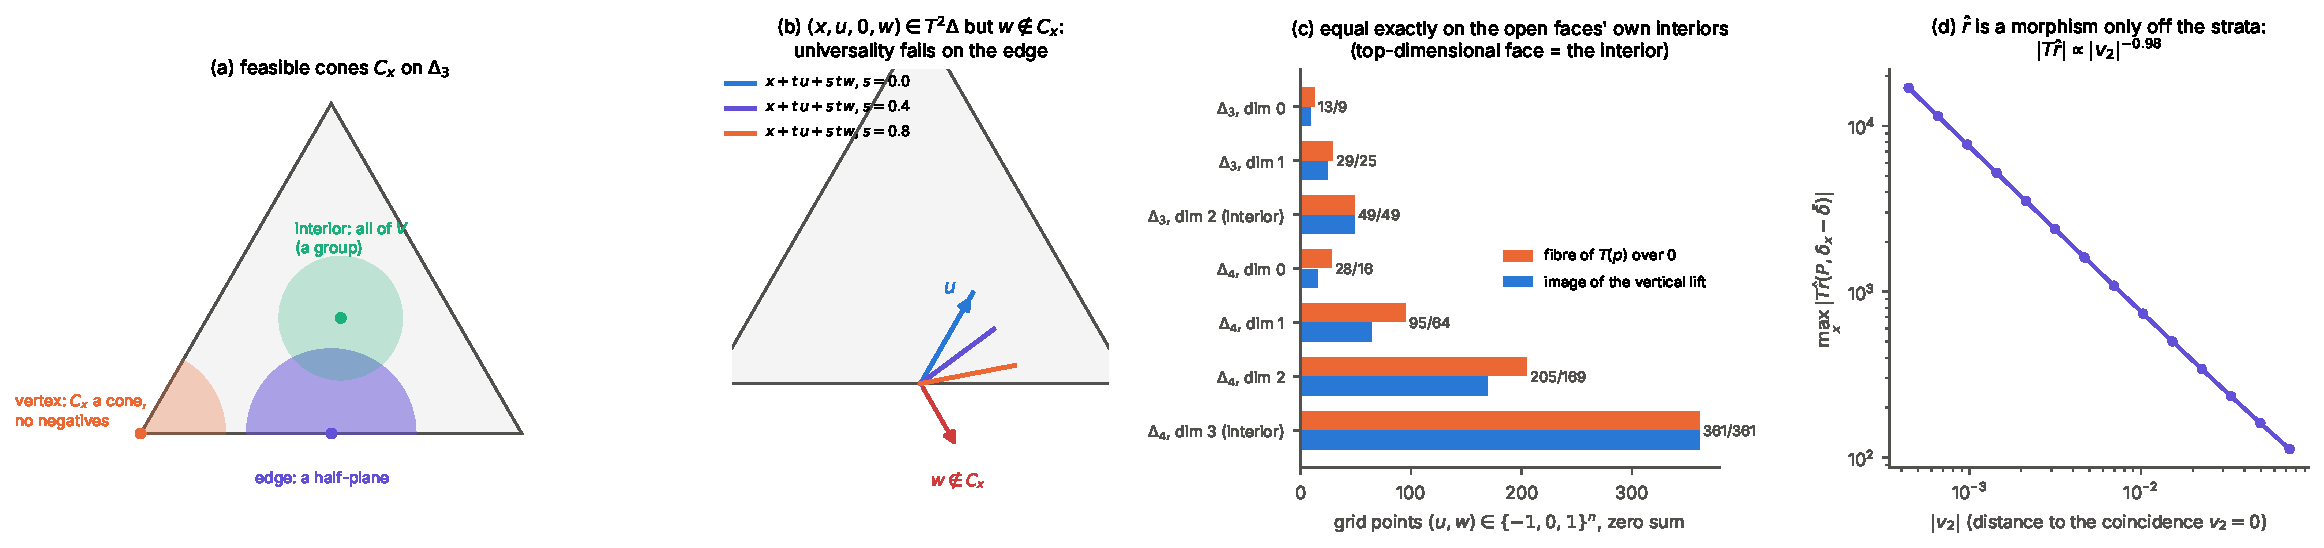
\includegraphics[width=\textwidth]{fig_cones.pdf}
\caption{The cone structure. (a) Feasible cones on $\Delta_3$: a pointed cone at a vertex (no negatives), a half-plane on an edge, and
the whole tangent space inside. (b) The universality counterexample on the edge (\cref{ex:delta3}): $u$ enters the face, $w\notin C_x$
leaves it, and the family $x+tu+stw$ stays in $\Delta_3$, so $(x,u,0,w)\in T^2\Delta_3$. (c) Grid points of the fibre of $T(p)$ over $0$
against the image of $\nu$, by face dimension on $\Delta_3$ and $\Delta_4$. They agree only on the interior (TG6). (d) $|T\hat r|$
against the distance to the coincidence $v_2=0$: slope $-0.98$, the simple pole of \cref{prop:interior}(3).}\label{fig:cones}
\end{figure}

\begin{figure}[t]\centering
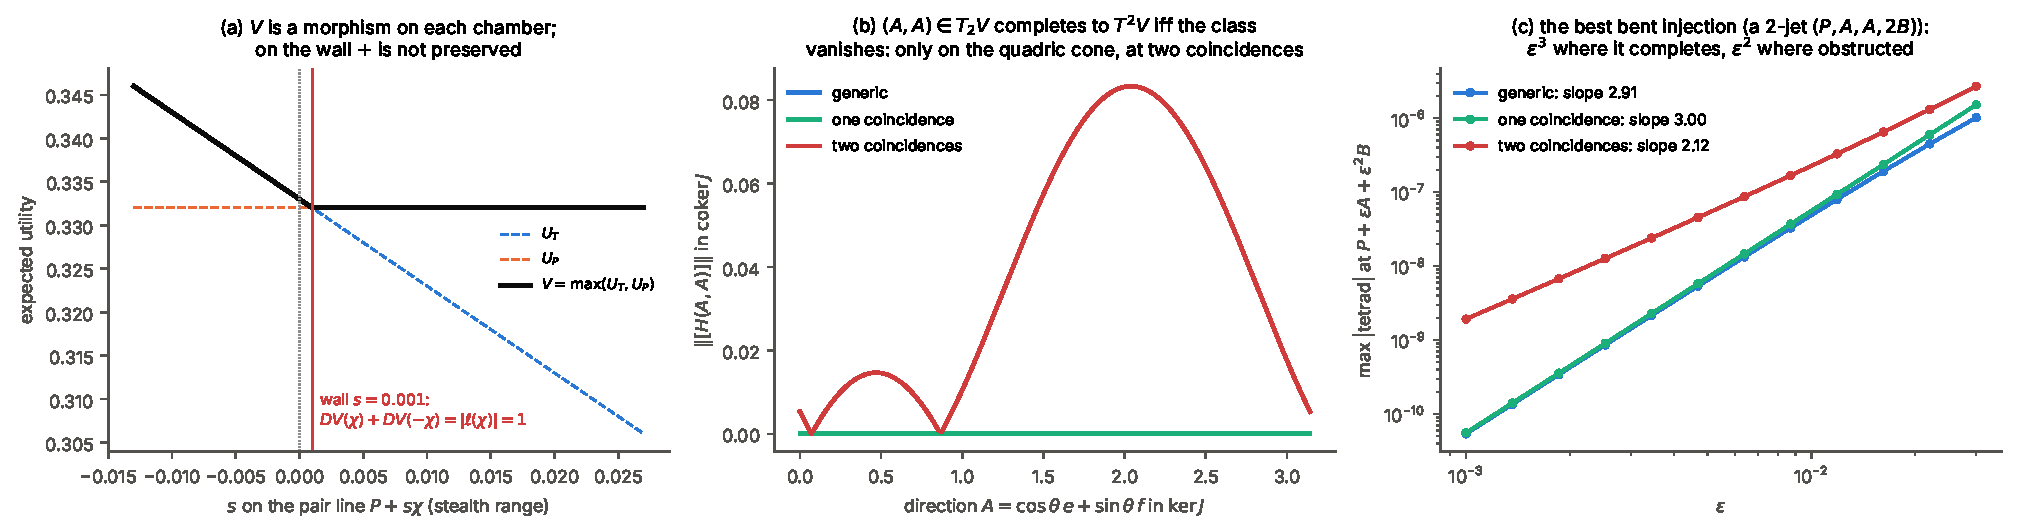
\includegraphics[width=\textwidth]{fig_jets.pdf}
\caption{Walls and jets. (a) The value function along the hidden channel $P+s\chi$ has a kink at the wall $s=0.001$, where
$DV(\chi)+DV(-\chi)=|\ell(\chi)|=1$ (\cref{prop:interior}(4)). (b) The completion class $\|[H(A,A)]\|$ around a circle of first-order
tetrad-stealthy directions. It vanishes identically at the generic and one-coincidence truths; at two coincidences it vanishes only
where the circle meets the quadric cone. (c) The tetrads at the best bent injection $P+\varepsilon A+\varepsilon^2B$, the 2-jet
$(P,A,A,2B)$: slope $3$ where the class vanishes, $2$ where it does not (\cref{thm:scheme}(3)).}\label{fig:jets}
\end{figure}

\section{Non-affine maps at corners: the second-order subcategory}\label{sec:nonaffine}
\Cref{prop:morph}(2) showed that a smooth map of simplices can fail to be a morphism of the cone structure at second order. The next
theorem says exactly which maps succeed. Write $C_x=L_x+\operatorname{cone}\{e_z-e_s\}$, where $L_x$ is the lineality space (the
directions inside the face of $x$) and $z$ runs over the empty cells of $x$, $s$ being a fixed cell of its support.

\begin{theorem}[second-order cone morphisms]\label{thm:nonaffine}
Let $f$ be smooth near $\Delta_n$ with $f(\Delta_n)\subseteq\Delta_p$, and $x\in\Delta_n$. Then $T^2f$ maps the fibre of $T^2\Delta_n$ over $x$
into $T^2\Delta_p$ iff, for every output cell $y$ with $f_y(x)=0$, the Hessian $H_y=D^2f_y(x)$ satisfies
\[
H_y(a,b)\ge0\qquad\text{for all }a,b\in K_y=C_x\cap\ker Df_y(x).
\]
Equivalently, $H_y$ vanishes on $L_x\times K_y$, and $H_y(r,r')\ge0$ for every pair of extreme rays $r,r'$ of $K_y$. These rays are the
$e_z-e_s$ with $\partial_zf_y(x)=\partial_sf_y(x)$. Pairs matter, not only the diagonal.
\end{theorem}

\begin{proof}
Write $\gamma=\nabla f_y(x)$. Since $f_y\ge0$ near $x$ on $\Delta_n$ and $f_y(x)=0$, $Df_y\ge0$ on $C_x$; so $\gamma$ is constant, say
$\gamma_0$, on the support, and $\gamma_z\ge\gamma_0$ on empty cells. The first-order conditions of \cref{lem:lex} for cell $y$ therefore
hold. The full condition, $(0,\,Df_yb,\,Df_ya,\,Df_yd+H_y(a,b))\lex0$, can fail only when $Df_ya=Df_yb=0$, that is $a,b\in K_y$. For
such $a$, $Df_ya=\sum_za_z(\gamma_z-\gamma_0)=0$ with non-negative terms, so $\gamma_z=\gamma_0$ wherever $a_z>0$; the same holds for $b$.
The admissible $d$ have $d_z\ge0$ on the empty cells where $a_z=b_z=0$ (\cref{lem:lex}), so
$Df_yd=\sum_zd_z(\gamma_z-\gamma_0)\ge0$, with equality at $d=0$. Hence the condition holds for all admissible $d$ iff
$H_y(a,b)\ge0$. Since $Df_y(e_z-e_s)=\gamma_z-\gamma_0\ge0$, $K_y=L_x+\operatorname{cone}\{e_z-e_s:\gamma_z=\gamma_0\}$. A bilinear form
that is non-negative on $K_y\times K_y$ must vanish on $L_x\times K_y$, because $\pm\ell\in K_y$ for $\ell\in L_x$.
\end{proof}

\begin{corollary}[the second-order subcategory]\label{cor:sub}
The maps satisfying \cref{thm:nonaffine} at every point form a subcategory, since $T^2$ is a functor. It contains:
\begin{itemize}
\item all stochastic matrices, for which $H=0$;
\item products of laws, whose Hessians have non-negative entries;
\item Bayesian conditioning $P\mapsto P(\cdot\mid A)$ on its domain $P(A)>0$.
\end{itemize}
The last is a partial map, a morphism of the restriction category of maps defined on relatively open subsets of the simplex
\cite{CockettCruttwellGallagher2011}; corners are included. On that subcategory the cone structure satisfies every axiom except (T6)
up to order two.
\end{corollary}

\begin{proof}
For conditioning, $f_y=P_y/P(A)$ with $y\in A$. At $P_y=0$ the gradient is $e_y/P(A)$, so every $a\in K_y$ has $a_y=0$. The Hessian is
$-\bigl(2a_yb_y+a_yb(A\setminus y)+b_ya(A\setminus y)\bigr)/P(A)^2$, which vanishes when $a_y=b_y=0$.
\end{proof}

On $60$ random quadratic self-maps of $\Delta_3$ at seven points each, the criterion and a direct test of $T^2f$ on sampled points of
$T^2\Delta_3$ agree in all $420$ cases, $29$ of which fail (TD1). For the counterexample of \cref{prop:morph}(2), $H_1(r,r)=2$ on both
rays but $H_1(r_1,r_2)=-2$. Copositivity alone would miss it; the theorem asks for bilinear non-negativity. The general order-$k$ condition
is presumably multilinear non-negativity of the $j$-th derivatives on these cones; we leave it open.

\section{Decision boundaries}\label{sec:decide}
The lab's decisions pass through estimators. The post-probe rule chooses T iff $F(P)=U_T(\hat r(P))-U_P>0$, which is smooth on the open
set $\{M_{01}M_{02}M_{12}>0\}$ (\cref{prop:interior}(3)) but not affine in $P$. The tangent structure computes what this costs.

\begin{proposition}[pooling paradox = curvature]\label{prop:pool}
Let $F$ be smooth on an open convex set, $F(P_0)=0$, $\nabla F(P_0)\ne0$, and let $\mathrm{II}=D^2F(P_0)|_{\ker DF}/|\nabla F|$ be the second
fundamental form of the boundary.
\begin{enumerate}
\item[(1)] If $\mathrm{II}(\xi,\xi)>0$ for a unit tangent $\xi$, then for small $\delta$ and $\eta=-c\delta^2$ with
  $0<c<\tfrac12\mathrm{II}(\xi,\xi)$, the laws $P_\pm=P_0\pm\delta\xi+\eta n$ ($n$ the unit normal) both have $F>0$, while their
  midpoint has $F<0$. If $\mathrm{II}(\xi,\xi)<0$, the same holds with the acts exchanged.
\item[(2)] If $F$ is affine in $P$, as the expected utility of a fixed act is, no mixture of two laws choosing the same act chooses the
  other.
\end{enumerate}
In injection terms, take $P_+$ as genuine data and $P_-$ as injected data. Each alone leads the decision maker to T, but the pooled data
lead to P.
\end{proposition}

\begin{proof}
(1) Expand $F(P_0+\delta\xi+\eta n)=\eta|\nabla F|+\tfrac12\delta^2D^2F(\xi,\xi)+O(\delta^3)$. With $\eta=-c\delta^2$ this is
$\delta^2|\nabla F|(\tfrac12\mathrm{II}(\xi,\xi)-c)+O(\delta^3)>0$ at both $P_\pm$, and $F(P_0+\eta n)=-c\delta^2|\nabla F|+O(\delta^4)<0$.
(2) A half-space is convex.
\end{proof}

\paragraph{On the lab.} Take the worked truth and the post-probe rule with the lab's acts, at the boundary point $P_0$ reached by moving the
truth $0.0021$ against the gradient.
\begin{itemize}
\item $\mathrm{II}$ has eigenvalues $-4.72,-2.92,-1.12,0.96,1.44,2.35$, so the boundary curves both ways (TD4).
\item With $\delta=0.02$, two laws with $F=9.6\cdot10^{-5}$ and $1.46\cdot10^{-4}$ (both choose T) have a mixture with $F=-1.16\cdot10^{-4}$
  (chooses P). Every injected share in $[0.14,0.85]$ flips the act. The reverse flip uses the most negative direction (TD5,
  \cref{fig:decide}).
\item For the affine decision functional, no flip occurs in $745$ random same-act pairs (TD6).
\end{itemize}
A screen that checks each source's data separately, asking whether it alone would lead to the same act, therefore certifies nothing about
the pooled decision. The curvature of the boundary is the obstruction. This is why the lab's gluing filter \cite[Theorem J]{Lab} tests
consistency between sources rather than the act each would choose.

\begin{proposition}[second-order budgets]\label{prop:budget}
For an injection direction $u=Q-P$, let $(F',F'')$ be the coefficients of $T^2F(P,u,u,0)$, so that
$F(P+\varepsilon u)=F+\varepsilon F'+\tfrac12\varepsilon^2F''+O(\varepsilon^3)$. The first-order budget is $\varepsilon_1=-F/F'$ (Theorem
E(3) of \cite{Lab}). The 2-jet budget $\varepsilon_2$ is the smallest positive root of the quadratic. Then $\varepsilon^*-\varepsilon_2=O(\varepsilon^3)$,
against $O(\varepsilon^2)$ for $\varepsilon_1$. The sign of $F''$ can reverse the first-order verdict either way. Along the hidden channel
$F''=0$ (the $e_1e_2$ coefficient of $T^2\hat r(P,\chi,\chi,0)$ is zero), so Theorem F's budget is exact.
\end{proposition}

\begin{proof}
Taylor's theorem along the line, and the implicit-function expansion of the root. Along $\chi$, $\hat r$ is affine
(\cref{sec:interior}), so $F$ is too.
\end{proof}

On the worked truth (TD7):
\begin{center}\small
\begin{tabular}{lcccp{0.36\textwidth}}\toprule
injected record & $\varepsilon_1$ & $\varepsilon_2$ & exact & note\\\midrule
$111$ & $0.002440$ & $0.002399$ & $0.002396$ & the vertex attack\\
$001$ & $0.010549$ & $0.010426$ & $0.010399$ & \\
$100$ & $0.013831$ & $0.013523$ & $0.013485$ & \\
$010$ & $0.4348$ & none & none & $F''>0$: the predicted flip never happens\\
$101$ & none & $0.0765$ & $0.4611$ & $F'>0$, $F''<0$: a harmless-looking record flips\\
hidden channel $\chi$ & $0.0010$ & $0.0010$ & $0.0010$ & $F''=0$: first order exact\\\bottomrule
\end{tabular}
\end{center}

\begin{figure}[t]\centering
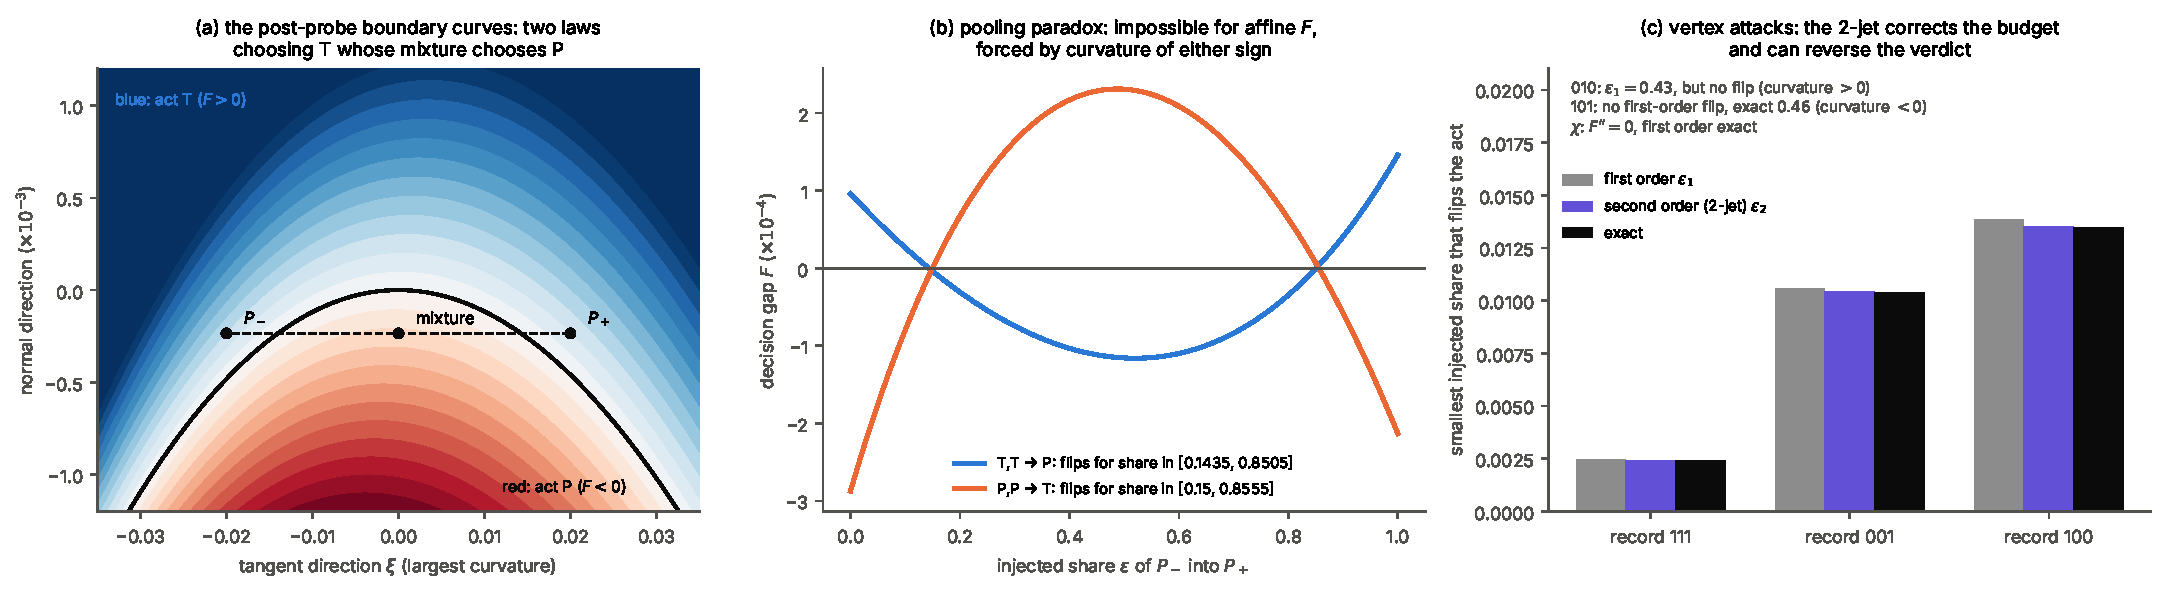
\includegraphics[width=\textwidth]{fig_decide.pdf}
\caption{Decision boundaries. (a) The lab's post-probe boundary $\{F=0\}$ in the plane through $P_0$ spanned by the normal and the most
curved tangent direction: two laws choosing T whose mixture chooses P. (b) The decision gap along both flip chords as a function of the
injected share. (c) Vertex-attack budgets: the 2-jet correction captures almost all of the first-order error.}\label{fig:decide}
\end{figure}

\section{Layers: restriction criteria at corners}\label{sec:layers}
\Cref{thm:nonaffine} treats a corner point with one cone. That is enough for smooth maps at second order, but near the boundary two
further things happen. First, the geometry can develop cusps and singular strata that the working dimension cannot resolve: a
projection loses what a lift would keep. Second, the map from data to explanations is many-valued, with sheets, continua and an empty
region. We therefore keep \emph{layered maps with restriction criteria}: three layers, each with its own criterion for where a map is
defined and smooth.

\begin{definition}[layered map]\label{def:layered}
\begin{enumerate}
\item[(1)] \emph{Strata.} A polyhedron is the disjoint union of its relatively open faces. Each face $F$ carries the restriction
  idempotent $e_F$, ``defined on $F$''. A layered map is a family $(f_F)$ of maps on the faces, compatible where closures meet: a join of
  restricted maps in the sense of \cite{CockettCruttwellGallagher2011}. Its restriction criterion on $F$ is \cref{thm:nonaffine},
  applied face by face.
\item[(2)] \emph{Resolutions.} A map that is singular on a stratum $S$ is replaced by its lift to a blow-up $\pi:\tilde X\to X$ along $S$,
  where it is smooth. The criterion records which chart of $\tilde X$ a point lies in.
\item[(3)] \emph{Multi-maps.} The explanation map is a correspondence $D\leftarrow\mathcal H\rightarrow\Theta$, from data to
  parameters through the hiding set. Its criteria are the existence conditions: gluing ($\lambda^*=1$), the sign class, the modulus class
  and positivity. Its branches are the sign sheets, and its tangent is the tangent cone of its graph.
\end{enumerate}
\end{definition}

The same layering applies to any polyhedron, in particular to the hiding sheets of the arbitrary-cover companion, whose layers are their
positivity walls (\cref{prop:restrictpoly}).

\begin{theorem}[layers resolve the corner]\label{thm:layers}
\begin{enumerate}
\item[(1)] Every relatively open face of a polyhedron, taken as its own object, has a universal vertical lift.
\item[(2)] At $x$ in a face $F$, a feasible direction $u$ enters the face $G(x,u)=\operatorname{supp}x\cup\{u>0\}\supseteq F$. The fibre
  of $T(p)$ over $0(x)$ is exactly
\[
\bigsqcup_{G\supseteq F}\{u\in C_x:G(x,u)=G\}\times C_G ,
\]
  with $C_G$ the cone at a relative-interior point of $G$. So the failure of universality in \cref{thm:cone}(4) is precisely a change
  of layer, and $C_{x,u}=C_{G(x,u)}$.
\item[(3)] The layered vertical bundle $\{(x,u,w):w\in C_{G(x,u)}\}$ is closed under the addition of $T(+)$, because $C_G$ grows with
  $G$ and $G(x,u+u')\supseteq G(x,u)\cup G(x,u')$.
\end{enumerate}
\end{theorem}

\begin{proof}
(1) In an open face all tangent directions are two-sided, as in the interior case. (2) By \cref{thm:cone}(4) the fibre is
$\{u\in C_x,\ w\in C_{x,u}\}$, and $w\in C_{x,u}$ iff $w_z\ge0$ for the cells with $x_z=u_z=0$, which are exactly the cells outside
$G(x,u)$. (3) Both inclusions follow from the definitions. Checks LY1--LY3 confirm all three by enumeration on $\Delta_3$ and $\Delta_4$.
\end{proof}

\begin{proposition}[the lab's resolutions and multi-maps]\label{prop:layers}
\begin{enumerate}
\item[(1)] \emph{Coincidence.} Downstairs $|T\hat r|$ grows like $1/|v_2|$ (\cref{prop:interior}(3)). Lifted to the parameters
  $(w,a_1,a_2)$ the same estimator is $r(w)=t-1/t$. Its derivative is bounded, and it vanishes in every $a$-direction (LY4). The parameter
  space is the resolution, and the singularity downstairs is the rank drop of the parametrisation (Theorem B of \cite{Lab}).
\item[(2)] \emph{Merge.} Families of truths with different weights entering the same product law keep $\hat r=r(w)$ constant all the way
  in, so $\hat r$ has no limit at the merge. In the blown-up coordinates $(\mu,\rho,\theta,t)$, with $v=\rho\theta$, the moments are
  $m_S=\rho^{|S|}\theta_Ss_{|S|}(r)$ and $\hat r=r$ is a smooth coordinate; the merge point has become the exceptional line $\rho=0$ (LY5).
  This is the lab's $n^{-1/4}$ tempo seen geometrically: the point that data space cannot resolve.
\item[(3)] \emph{The edge of the domain.} Scaling $c_{01}$ by $\lambda$ on the triangle moves the explanation segment. In $(\log\lambda,\log t)$
  the graph of the multi-map is a polygon with edges of slope $\pm\tfrac12$. It closes at a vertex at $\lambda^*=0.3115$, where
  positivity fails, so the tangent cone of the graph there is a wedge (LY6).
\item[(4)] \emph{Branches.} On two disjoint edges the relative-sign sheet shrinks and dies at $w^*=0.6231$ while the true sheet persists:
  a branch ends at a positivity wall (LY7).
\item[(5)] \emph{Criteria do not mix.} The pipeline's domain $\{M_{01}M_{02}M_{12}>0\}$ is not convex: two laws inside it can have
  mixtures outside it (shares $[0.400,0.458]$ in LY8). The pooling paradox of \cref{prop:pool} therefore needs the restriction criterion
  along the whole chord. A pooled data set can also simply fall outside the domain, so that the pipeline produces no decision at all.
\end{enumerate}
\end{proposition}

\begin{proof}
(1) $\hat r$ of an exact two-type law is its $r$ (Theorem F of \cite{Lab}), and $r$ depends on $w$ alone. (2) The same identity, applied
to the families $a_{1,2}=\mu\pm\rho\theta\,t^{\pm1}$. (3) By the hiding-polytope theorem of the arbitrary-cover companion the endpoints are minima and maxima of affine functions of
$\log|v_i|$, which are $\pm\tfrac12\log\lambda$ plus constants. (4) and (5) are computations (LY7, LY8).
\end{proof}

\begin{example}[a reader's guide to the layers, on $\Delta_3$ and the lab]\label{ex:layers}
\Cref{fig:layers} draws each layer.
\begin{enumerate}
\item \emph{Strata.} Take the edge point $x=(\tfrac12,\tfrac12,0)$ of \cref{ex:delta3}. The direction $u_1=(1,-1,0)$ stays on the edge, so
  its layer is the edge and the vertical directions must keep $w_3\ge0$. The direction $u_2=(-1,0,1)$ enters the interior, so any
  zero-sum $w$ is allowed. Over the grid, the corner fibre's $29$ points split as $15$ in the edge layer and $14$ in the interior layer
  (\cref{thm:layers}(2)). The naive pullback $T_2$ has only $5\times5=25$: it applies the edge's rule to every $u$.
\item \emph{Resolution.} Four two-type families with $w=0.6,0.3,0.45,0.75$ shrink to the same product law. Along each, $\hat r$ stays at
  $-0.408$, $+0.873$, $+0.201$ and $-1.155$ respectively, so at the merge the estimator has four different limits (panel b). Blown up
  (panel c), the merge becomes a line, and each family ends at its own point $r$ on it.
\item \emph{Multi-map.} Shrinking $c_{01}$ on the triangle narrows the band of explanations until it closes at $\lambda^*=0.3115$ (panel
  d). On two disjoint edges, the alternative labelling is possible only while $w<0.6231$ (panel e).
\item \emph{Mixing across the criteria.} Two laws on which the pipeline is defined can have mixtures on which it is not (panel f).
\end{enumerate}
\end{example}

\begin{figure}[t]\centering
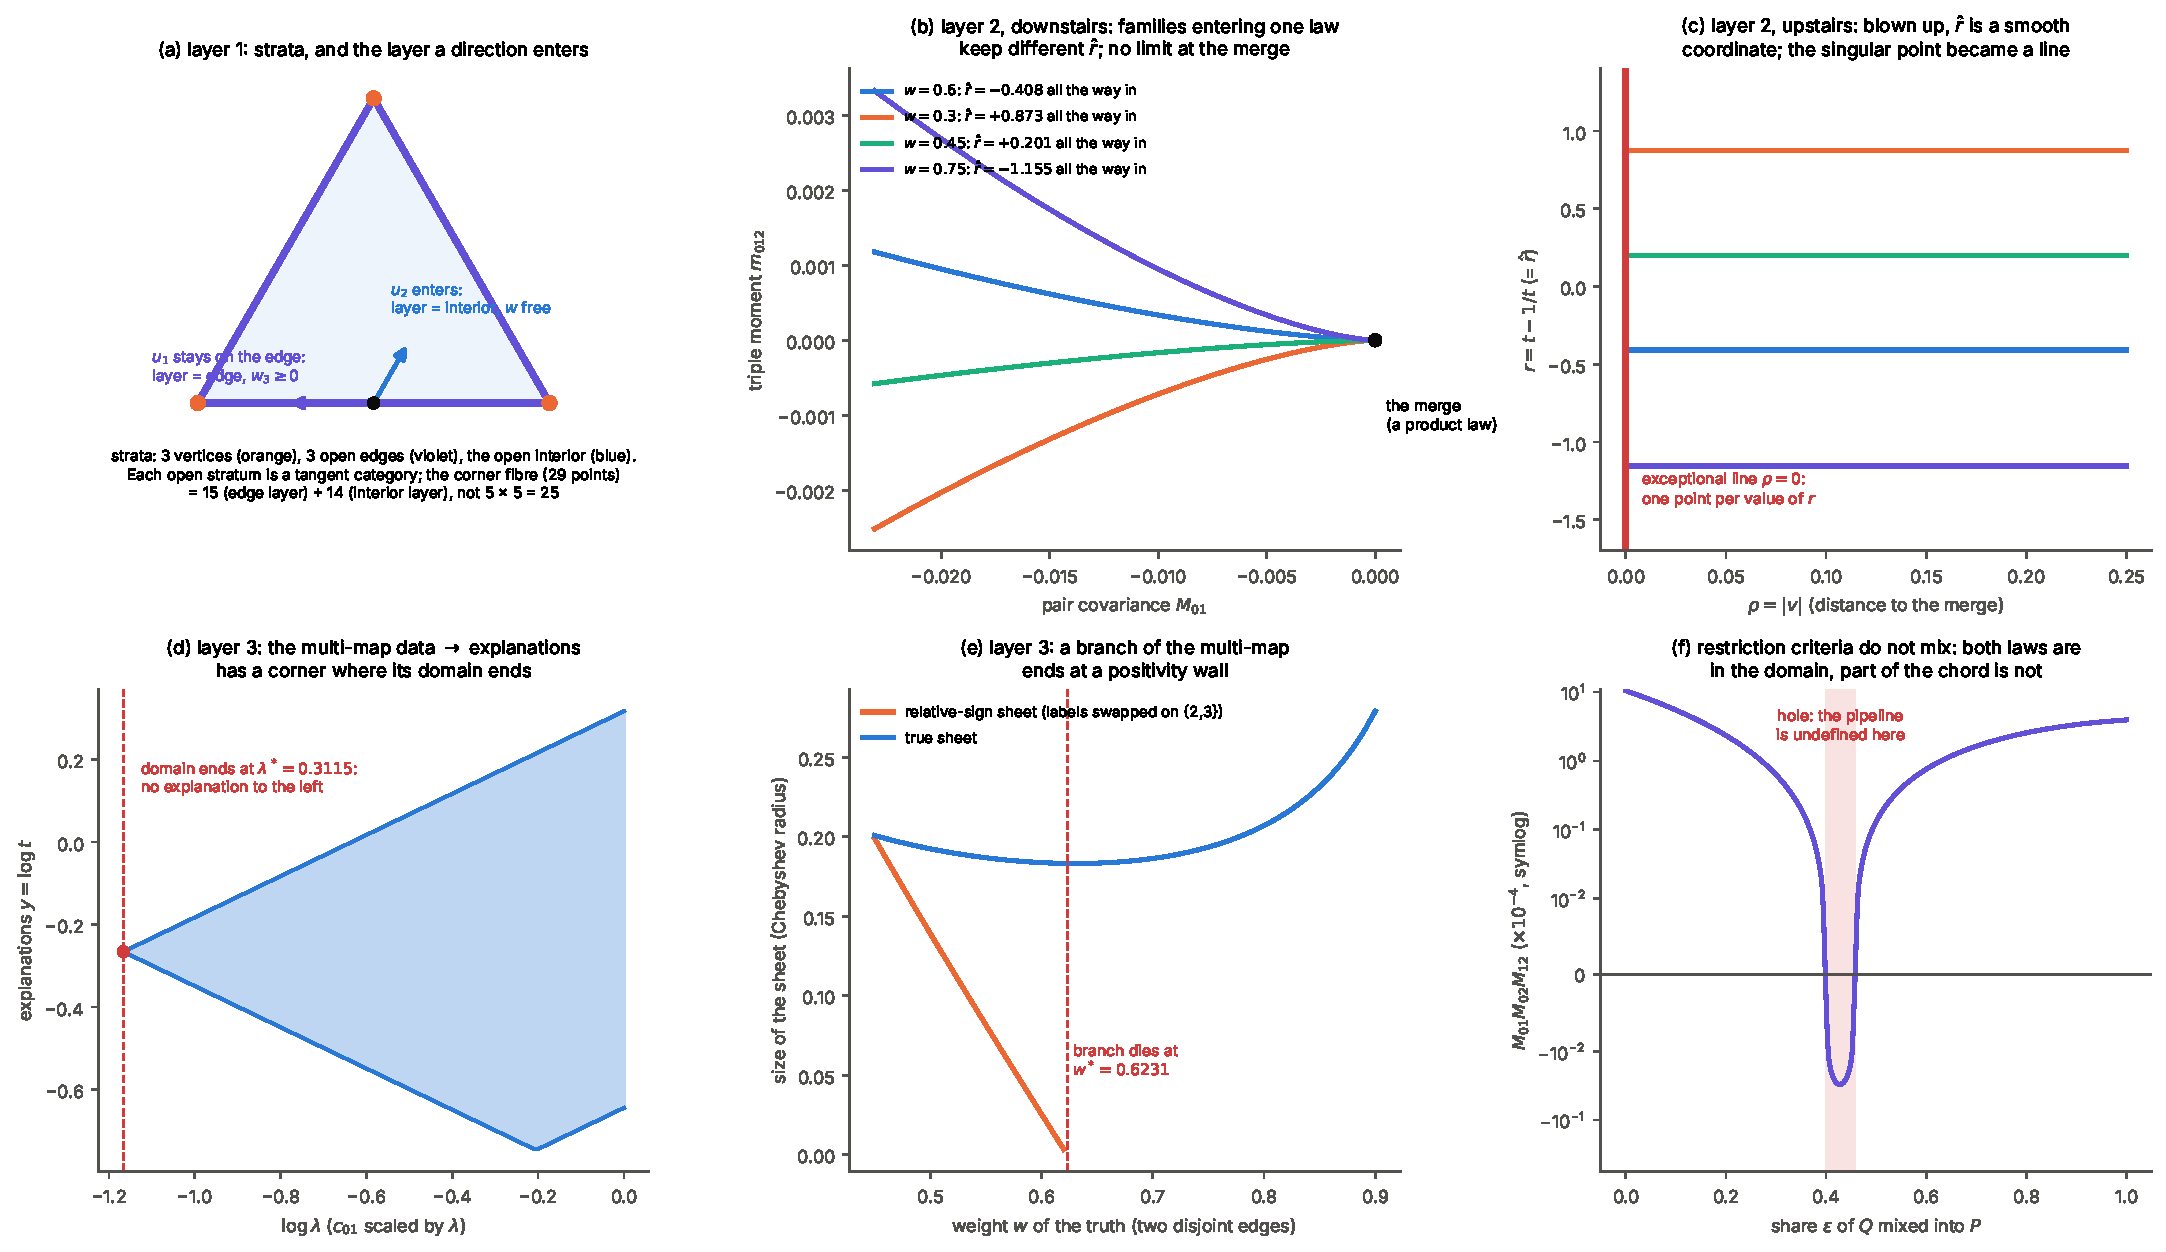
\includegraphics[width=\textwidth]{fig_layers.pdf}
\caption{Layers with restriction criteria (\cref{ex:layers}). (a) Strata of $\Delta_3$ and the layer a direction enters. (b)
Downstairs: families entering the merge keep different $\hat r$. (c) Upstairs: after the blow-up, $\hat r$ is a coordinate on the
exceptional line. (d) The explanation multi-map on the triangle: a polygon in $(\log\lambda,\log t)$ closing at the edge of its domain.
(e) A branch (the relative-sign sheet) ending at a positivity wall. (f) The pipeline's domain along a mixing chord.}\label{fig:layers}
\end{figure}

\section{The restriction structure, checked}\label{sec:restriction}
\Cref{cor:sub} and \cref{def:layered} used partial maps. Here we state the structure and check its axioms.

\begin{definition}[restriction category \cite{CockettLack2002}]\label{def:restriction}
A restriction category assigns to each map $f:A\to B$ an idempotent $\bar f:A\to A$, ``the domain of $f$'', such that
\begin{enumerate}[label=(R\arabic*)]
\item $f\bar f=f$;
\item $\bar f\bar g=\bar g\bar f$ for $f,g$ with the same source;
\item $\overline{g\bar f}=\bar g\bar f$;
\item $\bar gf=f\,\overline{gf}$ for composable $f,g$.
\end{enumerate}
Maps $f,g$ are \emph{compatible} if $f\bar g=g\bar f$. A join $f\vee g$ of compatible maps satisfies $\overline{f\vee g}=\bar f\vee\bar g$ and
$(f\vee g)h=fh\vee gh$ \cite{GuoThesis2012}. A tangent structure on a restriction category asks $T$ to be a restriction functor,
$T(\bar f)=\overline{Tf}$, with total natural structure maps \cite{CockettCruttwellGallagher2011,CockettCruttwell2014}.
\end{definition}

\begin{proposition}[the lab's restriction category]\label{prop:restriction}
Let $\mathcal R$ have simplices as objects and, as maps, partial maps $f$ that are defined on a relatively open subset of the source, are
smooth there, and satisfy \cref{thm:nonaffine} at every boundary point of their domain. Then:
\begin{enumerate}
\item[(1)] $\mathcal R$ is a restriction category with joins of compatible maps;
\item[(2)] $T$ is a restriction functor, $T(\bar f)=\overline{Tf}$ with $\operatorname{dom}Tf=T(\operatorname{dom}f)$, and the chain rule holds
  wherever composites are defined;
\item[(3)] its maps include the lab's partial maps: conditioning (domain $P(A)>0$), the post-probe estimator $\hat r$ (domain
  $M_{01}M_{02}M_{12}>0$), the decision gap, and the total maps (garblings, mixing). The value function is the join of $U_T$ on
  $\{F>0\}$ and $U_P$ on $\{F<0\}$; the wall is outside its domain.
\end{enumerate}
\end{proposition}

\begin{proof}
(1) The domain of $gf$ is $f^{-1}(\operatorname{dom}g)\cap\operatorname{dom}f$, relatively open by continuity. (R1)--(R4) hold for partial maps
of sets with $\bar f=\mathrm{id}_{\operatorname{dom}f}$. Smoothness is local, and the corner criterion is preserved by composition because $T^2$
is a functor on germs. Compatible maps agree on the intersection of their domains, so their join is defined on the union and is locally one
of them. (2) $Tf$ is defined at $(x,u)$ iff $x\in\operatorname{dom}f$, and the restriction of $Tf$ is $T$ of the restriction. (3) The maps are
smooth on their domains. Conditioning satisfies \cref{thm:nonaffine} (\cref{cor:sub}); the others have domains in the open simplex or are
affine.
\end{proof}

Checks RC1--RC4 verify (R1)--(R4) for conditioning, $\hat r$, a garbling and a mixing map on $600$ laws, including faces, corners and
points outside each domain. They also verify the join identities for the value function, the restriction-functor laws for $T$ with the
chain rule, and the corner criterion for conditioning at the corners $\delta_{000}$, $\delta_{001}$ and on the face $x_0=0$. We do not
attempt the full list of differential-restriction axioms; $T$ is checked as a restriction functor with total, natural structure maps.

\section{The tangent structure on a hiding sheet}\label{sec:sheets}
The companion on arbitrary covers describes the two-type explanations as sign sheets, polyhedra in $(\log t,\log\lambda)$ whose facets
are positivity walls \cite[Theorem 5]{Covers}. A sheet is therefore an object of the cone category (\cref{thm:cone}), its faces are its
layers (\cref{thm:layers}), and the explanation map from a sheet to the simplex is smooth. \emph{The tangent structure on the hiding
polytope is the tangent cone of the sheet}, and it governs robust decisions.

\begin{proposition}[restriction to the hiding polytope]\label{prop:restrictpoly}
Let $\Pi_\sigma=\{z:Az\le b\}$ be a sheet, in the coordinates $z=(\log t,\log\lambda)$ of \cite[Theorem 5]{Covers}.
\begin{enumerate}
\item[(1)] The tangent structure on $\Pi_\sigma$ is the restriction of the cone structure of \cref{thm:cone} along the affine inclusion
  $\Pi_\sigma\hookrightarrow\R^{1+b}$. The feasible directions at $z$ form the tangent cone $\{u:A_{\mathrm{act}(z)}u\le0\}$, and
  $T^k\Pi_\sigma$ is given by \cref{lem:lex} row by row.
\item[(2)] Every facet is a named positivity wall, $a_{1i}$ or $a_{2i}$ at $0$ or $1$. The layers of \cref{thm:layers} are the faces,
  that is, the sets of active walls.
\item[(3)] The vertical lift is universal at $z$ iff no wall is active there. So the universality failure on the boundary of
  $\Pi_\sigma$ is exactly the positivity wall.
\end{enumerate}
\end{proposition}

\begin{proof}
(1) The cone structure is defined on all lexicographic sets, and $T$ commutes with affine preimages (\cref{lem:interleave}). (2) Each row is
one of the four inequalities $0\le a_{ki}\le1$, written in logarithms \cite[Theorem 5]{Covers}. (3) This is \cref{thm:cone}(4) for the
polyhedron $\Pi_\sigma$. Check BR5 verifies the cone at a vertex (two walls, $a_{2,2}=0$ and $a_{2,3}=1$), on an edge and inside, against
the definition. Every active facet is a wall at $0$ or $1$, and the fibre counts of SH1 are $25/16$, $45/36$ and $81/81$.
\end{proof}

\begin{proposition}[decisions on a sheet]\label{prop:sheet}
\begin{enumerate}
\item[(1)] On a sheet the vertical lift is universal exactly at interior points (\cref{prop:restrictpoly}(3)).
\item[(2)] For a smooth decision functional $F$ on the laws, a worst case $z^*$ of $F\circ\mathrm{explain}$ over the sheet satisfies
  $DF(z^*)\cdot u\ge0$ for every $u$ in the tangent cone of the sheet at $z^*$, the first-order optimality condition of
  \cite[Theorem 6.12]{RockafellarWets1998}. Where this vanishes along a face, the second-order criterion of that layer decides.
\item[(3)] As the data move, each facet keeps its normal and shifts, because the right-hand sides are logarithms of moments. So the
  tangent of the explanation multi-map is a vector of facet shifts.
\end{enumerate}
\end{proposition}

\begin{proof}
(1) is \cref{thm:cone}(4) for a polygon (SH1). (2) is the standard first-order condition: the sheet is a polyhedron, so its tangent cone
equals its feasible cone. (3) The normals come from the incidence structure, not from the data \cite[Theorem 5]{Covers}. The shifts are
derivatives of $\log\mu_i$, $\log(1-\mu_i)$ and $\log|v_i|$ (SH3).
\end{proof}

On the $C_4$ example the worst case of $P(x_0=x_1=x_2=1)$ over the sheet is $0.0511$. It sits at the vertex where variable $3$'s two
walls meet, and the cone condition holds there (SH2; \cref{fig:global}(a)). Theorem L of the lab (settling iff the hiding segment lies in
one chamber) extends from segments to sheets: a decision is settled iff $F$ keeps its sign on the sheet, and the sign of $F$ at a vertex is
decided by the cone of that vertex.

\section{Global pooling}\label{sec:global}
\Cref{prop:pool} is local: it builds flips from curvature at a boundary point. Two arbitrary laws are a different matter. Their chord can
leave the pipeline's domain (\cref{prop:layers}(5)), so the restriction criterion must hold along the whole chord. For the post-probe rule
``T iff $\hat r>r_c$'' everything along a chord is polynomial, and the question can be decided exactly.

\begin{theorem}[pooling along a chord]\label{thm:global}
Let $P_\varepsilon=(1-\varepsilon)P+\varepsilon Q$, $q(\varepsilon)=M_{01}M_{02}M_{12}$ and $h(\varepsilon)=m_T^2-r_c^2q$.
\begin{enumerate}
\item[(1)] $\deg q\le6$ and $\deg h\le6$. The pipeline is defined on $\{q>0\}$, at most four intervals of $[0,1]$.
\item[(2)] The act can change only at the roots of $h$ where $q>0$ and $m_T=-r_c\sqrt q$ (the branch the squaring loses), so at most six
  times along any chord.
\item[(3)] \emph{Certificate.} If $P$ and $Q$ choose the same act and neither $q$ nor $h$ has a root in $(0,1)$ (Sturm counts), every
  mixture is defined and chooses that act. Isolating the roots decides every chord exactly.
\item[(4)] \emph{Holes force flips.} At an edge of a hole with $m_T\ne0$, $\hat r=m_T/(-\sqrt q)\to\mp\infty$. So near the edge the act is
  forced: T iff $m_T<0$. When this disagrees with the endpoints' act, the chord must flip on the way to the hole.
\item[(5)] \emph{Leaving the domain is a sign class.} $q<0$ means the pooled pair covariances have a negative product: the odd-cycle sign
  class of \cite[Theorem 14]{Covers}. The pooled data then have no two-type explanation at all, although each part has one.
\end{enumerate}
\end{theorem}

\begin{proof}
(1) Along a chord the means are linear in $\varepsilon$, the pair covariances are quadratic and $m_T$ is cubic. A polynomial of degree
$\le6$ splits $[0,1]$ into at most seven sign intervals, at most four of them positive. (2) $\hat r=r_c$ iff $m_T=-r_c\sqrt q$, which implies
$h=0$. (3) By continuity the act is constant on each interval between consecutive critical points. (4) $v_T\to0$ while $m_T$ stays
bounded away from zero. (5) A real two-type factorisation needs a positive product around the triangle \cite[Theorem 2]{Covers}.
\end{proof}

Checks GP1--GP4 confirm this on $650$ chords.
\begin{itemize}
\item The degrees are at most $6$ ($6$ and $6$ attained), and dense scans never exceed the root counts.
\item The certificate is never wrong. Between consecutive critical points the act is constant, and it changes exactly at the genuine roots.
\item \emph{The global picture.} Among same-act pairs, all $150$ within $0.02$ of the worked law are safe. At distance $0.06$, $78$ are safe and
  $72$ leave the domain; for pairs drawn anywhere, $43$ are safe and $107$ leave it. None of the $450$ pairs flips inside a single domain
  interval.
\end{itemize}
So, globally, pooling fails by leaving the domain: the pooled data acquire the liar's sign class. The flips that do occur sit next to the
holes, as (4) says (\cref{fig:global}(b)). The curvature flips of \cref{prop:pool} are real but need pairs placed near the boundary.

\begin{figure}[t]\centering
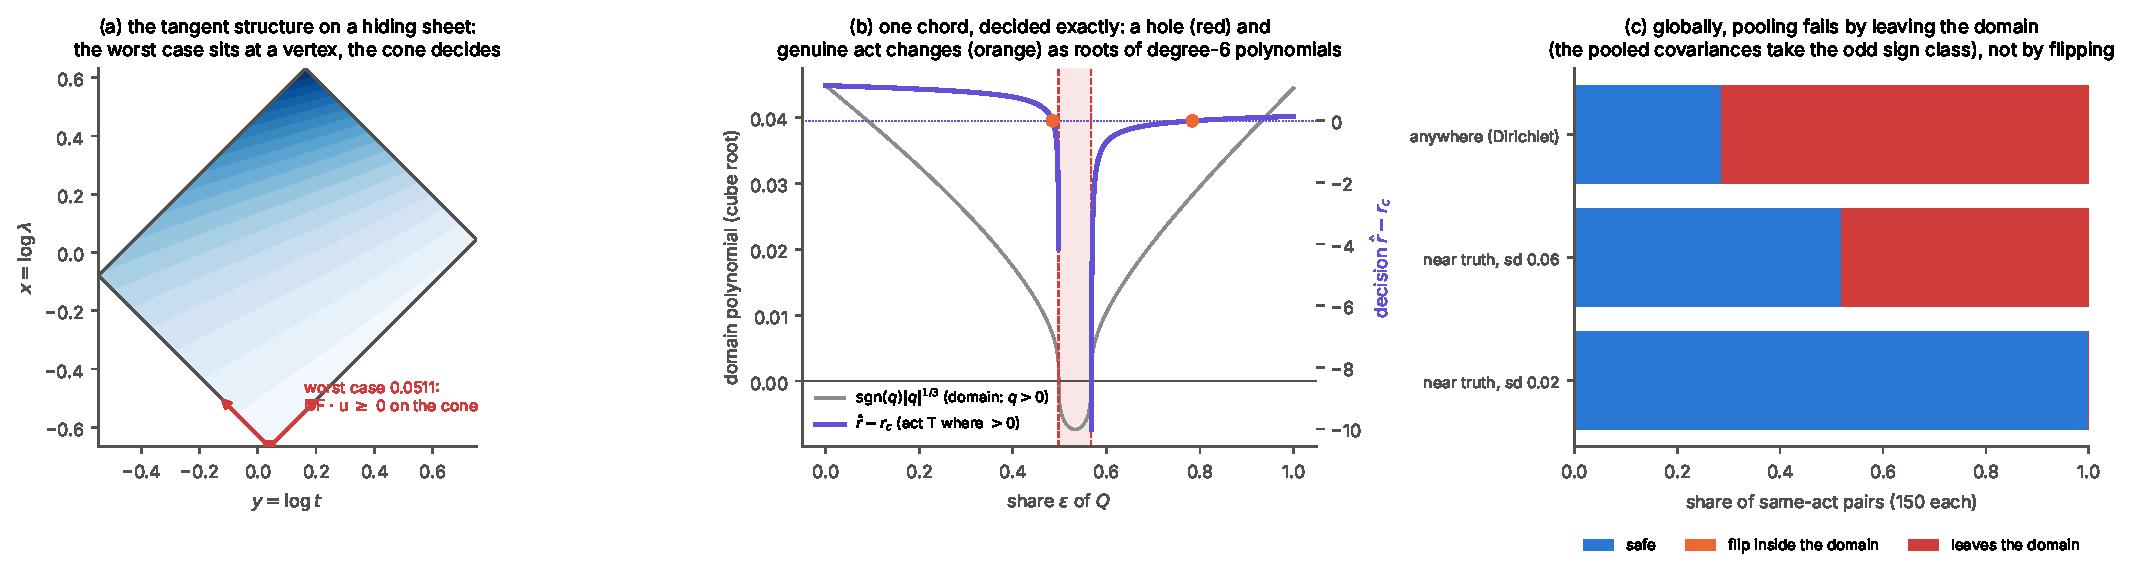
\includegraphics[width=\textwidth]{fig_global.pdf}
\caption{Sheets and global pooling. (a) The $C_4$ hiding sheet with the values of $P(x_0=x_1=x_2=1)$: the worst case sits at a vertex, and
the vertex's tangent cone certifies it. (b) One chord decided exactly: a hole where $q<0$ (red), $\hat r$ diverging at its edges, and the two
genuine act changes (orange) that the hole forces. (c) Same-act pairs at three distances from the truth: safe, flipping inside the domain,
or leaving it.}\label{fig:global}
\end{figure}

\section{Worked examples}\label{sec:worked}
\begin{example}[$\Delta_3$, every intermediate step]\label{ex:delta3}
\emph{The cone at an edge point.} Take $x=(\tfrac12,\tfrac12,0)$. Its cone is $C_x=\{u:\sum u=0,\ u_3\ge0\}$, a half-plane. Of the seven
zero-sum vectors in $\{-1,0,1\}^3$, five lie in it: $0$, $\pm(1,-1,0)$, $(-1,0,1)$ and $(0,-1,1)$.

\emph{A point of $T^2\Delta_3$.} Take $X=x+u\,e_1+0\,e_2+w\,e_1e_2$ with $u=(-1,0,1)$ and $w=(0,1,-1)$. In the size order
$(1,e_2,e_1,e_1e_2)$ the cells read:
\begin{center}\small
\begin{tabular}{lcccc}\toprule
cell & $U=\{1,2\}$: $(c_\varnothing,c_2,c_1,c_{12})$ & $U=\{1\}$: $(c_\varnothing,c_1)$ & $U=\{2\}$: $(c_\varnothing,c_2)$ & verdict\\\midrule
1 & $(\tfrac12,0,-1,0)$ & $(\tfrac12,-1)$ & $(\tfrac12,0)$ & $\lex0$ (leading $\tfrac12$)\\
2 & $(\tfrac12,0,0,1)$ & $(\tfrac12,0)$ & $(\tfrac12,0)$ & $\lex0$\\
3 & $(0,0,1,-1)$ & $(0,1)$ & $(0,0)$ & $\lex0$ (leading $1$ at $e_1$)\\\bottomrule
\end{tabular}
\end{center}
The column sums are $1,0,0,0$, so $X\in T^2\Delta_3$, and $T(p)X=(x,0)=0(x)$.

\emph{Not in the image of $\nu$.} $\nu^{-1}(X)$ would be $(x,w,u)\in T_2\Delta_3$, which needs $w\in C_x$, but $w_3=-1<0$. The realising
family $x+tu+stw=(\tfrac12-t,\ \tfrac12+st,\ t(1-s))$ lies in $\Delta_3$ for $0\le s<1$ and small $t$: cell $3$ is filled at rate $t$ and
drained at rate $st$.

\emph{Counting the fibre.} Over the grid, $\nu$ hits $5\times5=25$ pairs $(u,w)$. In the fibre, the three $u\in C_x$ with $u_3=0$ allow
$w\in C_x$ ($3\times5=15$), and the two with $u_3=1$ allow all seven $w$ ($14$), for $29$ in all. At the vertex $(1,0,0)$, $C_x$ has
three grid points and $\nu$ hits $9$. The fibre has $3+5+5=13$: $u=0$ gives $w\in C_x$, and each of the two edge directions frees the
other empty cell's sign. At the interior the two counts agree at $49=7^2$ (\cref{fig:cones}(c)).
\end{example}

\begin{example}[$\Delta_4$: the agreement table and its marginal]\label{ex:delta4}
Let $\Delta_4$ be the $2\times2$ tables, cells ordered $00,01,10,11$, and take the agreement table $x=(\tfrac12,0,0,\tfrac12)$, one of the
liar cycle's tables in the lab.
\begin{enumerate}
\item The injection cone is $C_x=\{u:\sum u=0,\ u_{01}\ge0,\ u_{10}\ge0\}$, three-dimensional with two facets.
\item The row marginal is the stochastic matrix $R=\begin{pmatrix}1&1&0&0\\0&0&1&1\end{pmatrix}$, a morphism of $\C$, with $T(R)(x,u)=(Rx,Ru)$.
  Its vertical bundle at $x$ is $\{u\in C_x:Ru=0\}=\{(-\alpha,\alpha,\beta,-\beta):\alpha,\beta\ge0\}$, a quadrant. The marginal-preserving
  injections at the agreement table can only create disagreement, never remove it.
\item Universality fails. With $u=(-1,1,0,0)$, which creates disagreement on $01$, take $w=-u=(1,-1,0,0)$. Then
  $(x,u,0,w)\in T^2\Delta_4$: cell $01$ reads $(0,0,1,-1)\lex0$. But $w\notin C_x$. Over the grid the fibre has $95$ points and the image
  $64$ on this edge, against $28$ and $16$ at a vertex, $205$ and $169$ on a 2-face, and $361=361$ inside.
\item The flip $c$ maps $(x,u,v,0)\mapsto(x,v,u,0)$ for any $u,v\in C_x$, and both are in $T^2\Delta_4$, as \cref{thm:cone}(1) requires
  (TG4 tests $7547$ applications of the structure maps at all face types, with no violation).
\end{enumerate}
\end{example}

\begin{example}[the lab's truth]\label{ex:lab}
For the worked law $P$ of \cite[Section 17]{Lab}, $P(001)=0.127$, the stealth range is $[-0.013,0.027]$, and the decision gap is
$U_T-U_P=0.128-P(001)$, with $\ell=u_T-u_P$ and $\ell(\chi)=-1$. The single-record influences of $\hat r$ are $T\hat r(P,\delta_x-P)=5.15$
($x=000$), $-14.93$ ($001$) and $-64.54$ ($111$). The hidden-channel slope is $T\hat r(P,\chi)=1/v_T=-157.50$. At $s=0.001$ the act changes; there
$DV$ ceases to be additive with defect $|\ell(\xi)|$, while inside the chamber the defect is $0$ to $10^{-6}$ on random $\xi$.
\end{example}

\section{What this answers, and what it does not}\label{sec:answers}
\begin{itemize}
\item \emph{Built, not named.} The objects (lexicographic sets; open simplices; the tetrad scheme), the functor and the five
  transformations are explicit, and every axiom is verified. The one axiom that fails, universality at corners, fails with a proof, an
  explicit counterexample and an exact description of the fibre.
\item \emph{The lab's named structures become tangent-categorical ones.} The influence function is $T(F)$ at the injection direction.
  The stealth directions are the vertical bundle of the marginal map. The André--Quillen obstruction is the failure of $T^2V\to T_2V$ to
  be onto, with Theorem G(4)'s class as its diagonal. The wall is where the value function stops preserving $+$.
\item \emph{Scope.} Simplices, polyhedra and affine maps at the boundary; smooth maps in the interior; the two-type tetrad scheme at
  $m=4$. Non-affine maps at corners are settled at second order by \cref{thm:nonaffine}; the order-$k$ condition is open. The two-type
  theory on arbitrary covers, with the three-type proof of concept, is the other companion.
\item \emph{Used, not only built.} On decision boundaries the structure computes three new things. It gives the exact class of maps
  allowed at corners. It shows that curvature of the boundary forces a pooling paradox, which affine decisions cannot have. And it gives
  second-order attack budgets, which can reverse first-order verdicts.
\end{itemize}

\section*{Checks}
\begin{sloppypar}
\begin{itemize}
\item The structure: \texttt{engine/check\_tangent.py} (module \texttt{engine/pce/tangent.py}; $14/14$, about one minute).
\item Decision boundaries: \texttt{engine/check\_tangent\_decide.py} (module \texttt{engine/pce/tangent\_decide.py}; $7/7$).
\item Layers: \texttt{engine/check\_layers.py} (module \texttt{engine/pce/layers.py}; $8/8$).
\item Restriction, sheets and pooling: \texttt{engine/check\_restriction.py} (module \texttt{engine/pce/restriction.py}; $11/11$).
\end{itemize}
\end{sloppypar}
\begin{center}\small
\begin{tabular}{lp{0.78\textwidth}}\toprule
TG1 & Weil arithmetic exact: $T$, $T^2$ of $\hat r$, of the decision gap and of the tetrads against finite differences; Schwarz symmetry\\
TG2 & the lexicographic lemma against the definition, exhaustively for $k=1,2,3$\\
TG3 & the eleven equational axioms as substitution identities\\
TG4 & structure maps preserve $T^k\Delta$ on $\Delta_3$, $\Delta_4$ at every face type; monoid; negatives only inside\\
TG5 & stochastic matrices and products preserve $T^k\Delta$; the non-affine counterexample\\
TG6, TG6b & universality iff relative interior: $\Delta_3$, $\Delta_4$ and a cut cube, with the fibre $C_x\times C_{x,u}$\\
TG7 & the edge counterexample and its realising family\\
TG8 & $T F(P,Q-P)=\sum_xQ(x)\mathrm{IF}(x)$; the pole of $T\hat r$ at a coincidence\\
TG9 & stealth directions are vertical; the rays at the ends of the stealth range\\
TG10 & the wall's additivity defect $|\ell(\xi)|$; $1$ along $\chi$\\
TG11 & universality on the tetrad scheme at all three truths\\
TG12 & completion: onto off the stratum; class $|q|/\sqrt2$ on it; diagonal $=2\,\mathrm{ob}$; onto on the cone side\\
TG13 & 2-jets: bent-injection slopes $3$, $3$, $2$\\\midrule
TD1 & the Hessian criterion equals the direct $T^2$ test ($420/420$); the counterexample fails on a ray pair only\\
TD2, TD3 & stochastic maps, products and conditioning pass; composites pass; conditioning as a partial map\\
TD4 & the post-probe boundary has curvature of both signs\\
TD5 & mixture flips both ways, for shares in $[0.14,0.85]$\\
TD6 & affine decisions never flip\\
TD7 & second-order budgets; curvature reversals for $010$ and $101$; the hidden channel exact\\\midrule
LY1--LY3 & open faces universal; corner fibre $=$ union over entered layers; the layered bundle closed under $+$\\
LY4, LY5 & resolutions: the coincidence lifted to the parameters; the merge blown up\\
LY6, LY7 & the multi-map: a corner at the edge of its domain; a branch dying at a positivity wall\\
LY8 & the pipeline's domain is not convex\\\midrule
RC1--RC4 & restriction axioms R1--R4, joins, $T$ a restriction functor, the corner criterion on its domain\\
SH1--SH3 & sheets: universality inside only; worst case and cone condition; facet shifts\\
GP1--GP4 & pooling along chords: degrees, root bounds, the certificate, the exact decision and the global picture\\
BR5 & restriction to the hiding polytope: tangent cone, walls as facets, universality fails exactly on walls\\\bottomrule
\end{tabular}
\end{center}

\begin{thebibliography}{99}
\bibitem{Lab} V.~K.~Awasthi, A lab for latent actors: hiding segments, probes, settled decisions, injected records and sources, 2026.
\bibitem{CockettCruttwell2014} J.~R.~B.~Cockett and G.~S.~H.~Cruttwell, Differential structure, tangent structure, and SDG, \emph{Appl. Categ. Structures} \textbf{22} (2014) 331--417.
\bibitem{CockettLack2002} J.~R.~B.~Cockett and S.~Lack, Restriction categories I: categories of partial maps, \emph{Theoret. Comput. Sci.} \textbf{270} (2002) 223--259.
\bibitem{Covers} V.~K.~Awasthi, Two latent types on arbitrary covers, companion paper, 2026.
\bibitem{GuoThesis2012} X.~Guo, \emph{Products, Joins, Meets, and Ranges in Restriction Categories}, PhD thesis, University of Calgary, 2012.
\bibitem{CockettCruttwellGallagher2011} J.~R.~B.~Cockett, G.~S.~H.~Cruttwell and J.~D.~Gallagher, Differential restriction categories, \emph{Theory Appl. Categ.} \textbf{25} (2011) 537--613.
\bibitem{Danskin1967} J.~M.~Danskin, \emph{The Theory of Max-Min and its Application to Weapons Allocation Problems}, Springer, 1967.
\bibitem{Fritz2020} T.~Fritz, A synthetic approach to Markov kernels, conditional independence and theorems on sufficient statistics, \emph{Adv. Math.} \textbf{370} (2020) 107239.
\bibitem{Garner2018} R.~Garner, An embedding theorem for tangent categories, \emph{Adv. Math.} \textbf{323} (2018) 668--687.
\bibitem{KolarMichorSlovak1993} I.~Kolář, P.~W.~Michor and J.~Slovák, \emph{Natural Operations in Differential Geometry}, Springer, 1993.
\bibitem{Leung2017} P.~Leung, Classifying tangent structures using Weil algebras, \emph{Theory Appl. Categ.} \textbf{32} (2017) 286--337.
\bibitem{Rosicky1984} J.~Rosický, Abstract tangent functors, \emph{Diagrammes} \textbf{12} (1984).
\bibitem{RockafellarWets1998} R.~T.~Rockafellar and R.~J.-B.~Wets, \emph{Variational Analysis}, Springer, 1998.
\bibitem{Weil1953} A.~Weil, Théorie des points proches sur les variétés différentiables, \emph{Colloque de Géométrie Différentielle}, Strasbourg, CNRS, 1953, 111--117.
\end{thebibliography}
\end{document}
